%*******************************************************************************
%*********************************** First Chapter *****************************
%*******************************************************************************

\chapter{Introduction: The Aim Of VIDARR} \label{Chap:theAimOfVidarr} %Title of the First Chapter
The aim of the VIDARR project is to demonstrate the potential usefulness of a plastic scintillating detector for safeguarding purposes. To that end the characterisation and simulation of two versions of the detector will be used in order to show the full potential of this idea. Reactor monitoring using $\Bar{\nu_e}$ was suggested as early as 1978 \cite{Borovoi_1978} but the political climate of the cold war era prevent interest in the technology from being fully realised. In the modern political climate where nuclear power is seen as a stable form of low carbon power generation more nations are considering the technology once again. And as such the concern of the proliferation of atomic weapons has increased. Current methods of non-proliferation are dependent on accurate bookkeeping and empirical measurement estimations from power generation. Whilst these methods are effective more direct methods of measuring the flux from reactors and thereby the production of weapons grade material would greatly aid in the trust between nations and help to prevent the spread of atomic weaponry. 
\\\\This technology also has benefits for increasing the burn-up of nuclear waste which could increase power generation at nuclear power plants and reduce the production of nuclear waste which has to be stored. This potential is not yet fully realised due to the increased complexity of the method as it requires differentiating between different isotopes rather than just measuring flux. Tough this should be feasible it is not possible to test this capability until the upgraded VIDARR detector is deployed at a reactor site. 

\section{Discovery of neutrinos}
\subsection{Theoretical Development}
%history of neutrino: \cite{griffiths2008neutrino1.5} \cite{lederman1970resource}
%\\beta decay of tritium (book cannot find, may have to replicate): \cite{lewis1970neutrinos} especially as Fermi mentions it in \cite{Fermi:1934hr}, \cite{wilson1968fermi} 
%\\Neutron proposed by Chadwick in 1932 describing a proton like recoil and odd behaviour of neutrons that can only be described by a neutron or the breaking of conservation of momentum and energy!: \cite{chadwick1932possible}. Important for giving full context to the neutrino discovery
%\\Fermis paper proposing this beta decay after Chadwick's discovery of the neutron is given in \cite{Fermi:1934hr} which proposes a neutrino and is published through Springer and the English translation from 1968 is given in \cite{wilson1968fermi}
%\\So far very little from Pauli need to include him somewhere the neutrino was his idea \cite{lederman1970resource} may have something...
The neutrino was proposed as by Pauli in 1931 as a way to conserve the energy of $\beta$ decay and to conserve the angular momentum of the products of $\beta$ decay  \cite{griffiths2008book}\cite{griffiths2008neutrino1.5}\cite{lederman1970resource}. At the time beta decay was described by equation \ref{oldBetaDecay}. Where A and B represent the decaying particles, as the neutron had not yet been discovered by this point, it was considered a reaction between two nuclei. The conservation of energy dictates that the kinetic energy of the electron should only have a single value as shown in equation \ref{constant_ke_e_equation}. However, when the kinetic energy of the electron was measured \ref{beta_spectrum} the energy of the electron was not constant as seen in figure \ref{beta_spectrum} \cite{griffiths2008book} \cite{griffiths2008neutrino1.5} \cite{lewis1970neutrinos}. Equation \ref{constant_ke_e_equation} represents the maximum possible energy available to the electron in figure \ref{beta_spectrum} suggesting a third body in $\beta$ decay \cite{griffiths2008book} \cite{griffiths2008neutrino1.5}.


\begin{equation}
    A \rightarrow B + e^-
    \label{oldBetaDecay}
\end{equation}

\begin{equation}
    E = \left( \frac{{m_A}^2 - {m_B}^2 + {m_e}^2}{2m_A}\right) c^2
    \label{constant_ke_e_equation}
\end{equation}

\begin{figure}[htbp]
 \centering
 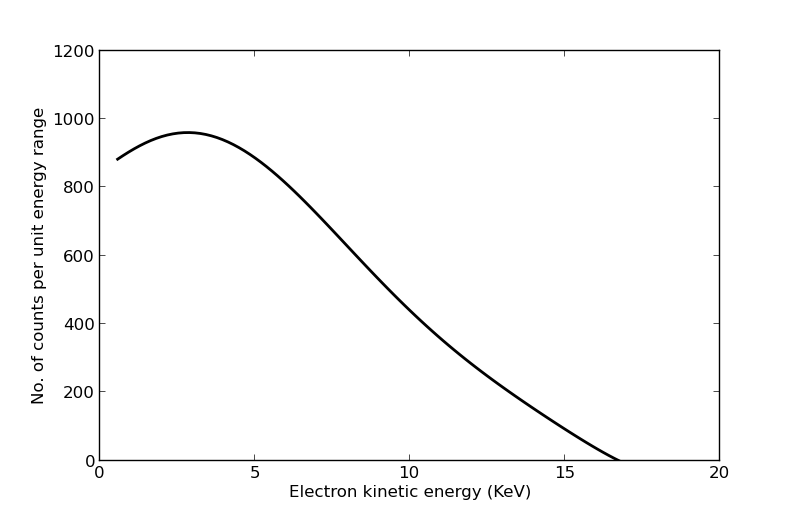
\includegraphics[height=90mm]{Chapter1/Figs/Raster/beta_spectrum.png}
 \captionof{figure}{$\beta$ spectrum reproduced from \cite{griffiths2008book}\cite{griffiths2008neutrino1.5} originally from \cite{lewis1970neutrinos}. The energy of the $e^-$ from $\beta$ decay varies significantly suggesting a 3 body decay model for $\beta$ decay instead of a 2 body model.} %~can be used as a kind of place holder in latex
 \label{beta_spectrum}
\end{figure}

The beta spectrum shown in figure \ref{beta_spectrum} was the first indirect evidence that neutrinos may exist. However Pauli waited until Chadwick's discovery of the neutron in 1932 \cite{chadwick1932possible} before publishing in 1934 \cite{lederman1970resource}. The complete picture of a proton-neutron nucleus allowed Enrico Fermi to produce a comprehensive theory of $\beta$ decay which incorporated Pauli's neutrino into $\beta$ decay \cite{lederman1970resource} \cite{Fermi:1934hr}. Note: a translation of Fermi's work was used \cite{wilson1968fermi}. This more complete picture made sure to differentiate the particles of the nucleus (protons and neutrons) with particles that were not bound to it (electrons and neutrinos) \cite{Fermi:1934hr} \cite{wilson1968fermi}. This period however leaves us with a mass-less neutrino which has spin 1/2 \cite{lederman1970resource}. The discovery of neutrino oscillations which will be mentioned later in section \ref{section_neutrino_oscillations} indicate that neutrinos do have mass but they were discovered far after this \cite{griffiths2008book} \cite{griffiths2008neutrino1.5}. The equation of $\beta$ decay was now given by equation \ref{semi_modern_beta_decay}. The discovery of lepton number and anti-netrinos had not yet been made however and so that quantity is not conserved in equation \ref{semi_modern_beta_decay}. 

\begin{equation}
    n \rightarrow p^+ + e^- + \nu
    \label{semi_modern_beta_decay}
\end{equation}

\subsection{Direct Measurements}\label{Direct_Measurements_section}
%propossal of cowan and riens using a large liquid scintillator detector: \cite{reines1953proposed}
%\\First detection: \cite{reines1953detection}
%\\distingiusing the neutrino and anti-neutrino \cite{davis1959attempt}
%\\Need to find cloud chamber pictures showing the conservation of momentum \cite{griffiths2008book} \cite{griffiths2008neutrino1.5} shows them, need to find direct source. \cite{griffiths2008book} \cite{griffiths2008neutrino1.5} also goes on to explain why this matters.
%\\ \cite{michel1949energy} supposedly does show this, but I'm having trouble getting my hands on it, UoL doesn't have access to nature papers! So will just have to include a picture from \cite{griffiths2008book} \cite{griffiths2008neutrino1.5} and clarifiy it is from \cite{michel1949energy}.
%\\ There is also the suggestion from cowan early on that anti-neutrinos and neutrinos are differing particles,  \cite{cowan1957test}, however this is by no means certain it is possible that neutrinos and anti-neutrinos are differing spin states of the same particle.
%\\ There is also the early suggestion of neutrinos and anti neutrinos being separated by a certain quantity suggested by \cite{konopinski1953universal} under a universal interaction. They use muons to suggest that certain reactions are not possible, this would later come to be known as lepton number. \\\\
%Suggestions of differing types of neutrino supposedly come from the Soviet union in 1960 but this has been lost to the iron curtain unfortunately I could not find the paper myself. The earliest reference I found is \cite{pontecorvo1963neutrino} in 1963 talking about how this influences astrophysics. 
%\\The direct measurement of differing types of neutrinos was done by \cite{DanbyG1962PhysRevLett.9.36} in 1962. This was done with a pion beam striking a beryllium target and a 10 ton spark chamber behind the target in order to pick up 37 events of one reaction and not another. They also make reference to kions but seem less certain about those due to experimental limitations. They call this the ``The neutrino flip hypothesis.'' This is a really important paper.\\

Experimental evidence for a neutrino had been observed as early as 1949, in figure \ref{pion_path} it is possible to see the impact of the neutrino. The neutrino itself is neutral and so does not show in the emulsion in figure \ref{pion_path} however the effect of the neutrino can be seen both in how the pion decays into a muon and how the muon decays into an electron \cite{griffiths2008book} \cite{griffiths2008neutrino1.5}. Collisions in the emulsion cannot account for the 90$^o$ change in direction as the particles decay, collisions can only account for dithering not abrupt changes in direction \cite{griffiths2008book} \cite{griffiths2008neutrino1.5}. At the time it was piratical to assume that the pion decay shown in equation \ref{pion_nolepNo_decay} and the muon decay shown in equation \ref{muon_nolepNo_decay} both produced the same particle when decaying. The neutrino $\nu$ \cite{griffiths2008book} \cite{griffiths2008neutrino1.5}. However as seen in equations \ref{pion_nolepNo_decay} and \ref{muon_nolepNo_decay} lepton number and neutrino flavour were not yet known and so were not conserved.
\begin{equation}
    \pi \rightarrow \mu + \nu
    \label{pion_nolepNo_decay}
\end{equation}
\begin{equation}
    \mu \rightarrow e^- + 2\nu
    \label{muon_nolepNo_decay}
\end{equation}
\\
\begin{figure}[htbp]
 \centering
 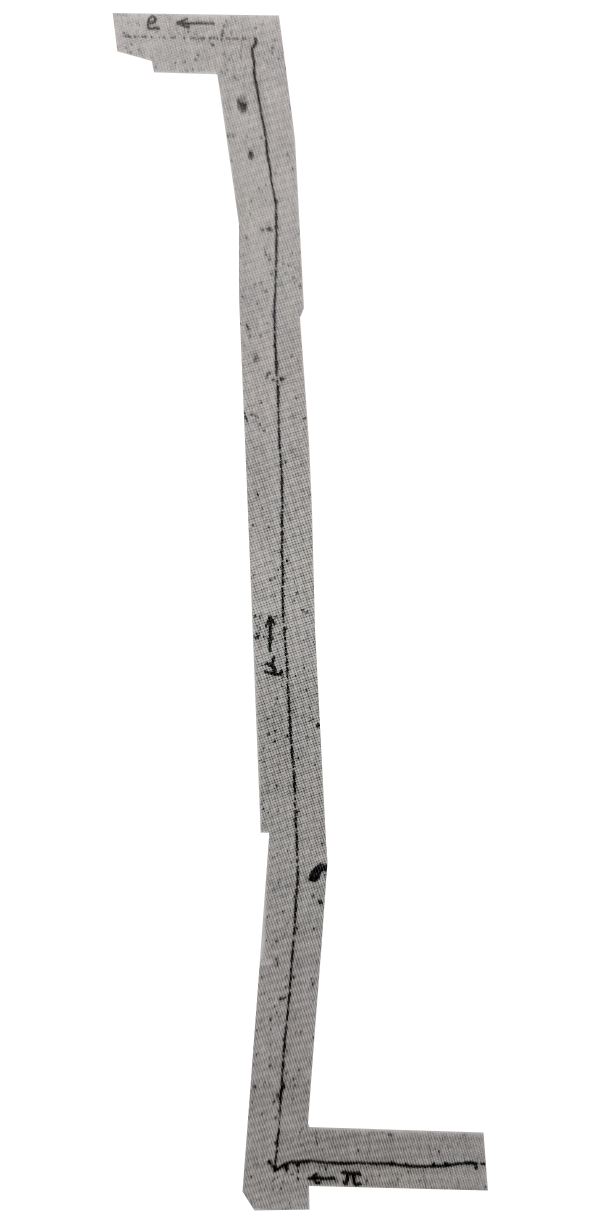
\includegraphics[height=90mm]{Chapter1/Figs/Raster/less_detailed_proper_path.png}
 \captionof{figure}{Path of pion decaying to a muon emitting one anti-neutrino (equation \ref{pion_nolepNo_decay}) and then that muon decaying into an electron emitting a neutrino and an anti-neutrino (equation \ref{muon_nolepNo_decay}). The paths at 90$^o$ show particle decay, collisions cannot account for this. From \cite{griffiths2008book} \cite{griffiths2008neutrino1.5} originally from \cite{michel1949energy}.} %~can be used as a kind of place holder in latex
 \label{pion_path}
\end{figure}
The first direct detection of a neutrino would be 22 years after it's initial proposal in 1931. In 1953 Cowan and Reines proposed a neutrino detector that used large amount of liquid scintillator to detect neutrinos \cite{reines1953proposed}. This proposal was followed up the same year with a cadmium loaded scintillation detector that used a delayed coincidence measurement allowing for the reduction of background \cite{reines1953proposed} \cite{reines1953detection}. The detector worked by looking for inverse $\beta$ decay shown in equation \ref{inverse_beta_decay}, though the different flavours of neutrinos were not yet known. The source of the neutrinos was a reactor at Hanford \cite{reines1953detection}. This resulted in a difference counting rates in the delayed time channels of 0.41 $\pm$ 0.20 counts/min due to the pile \cite{reines1953detection}. This result was later confirmed in 1956 at the Savanaah River Plant \cite{Cowan1956Confirmation}. This new detector used a combination of liquid scintillator in three layers and cadmium chloride doped water in another two layers in a ``club-sandwich'' arrangement. This resulted in an unambiguous measurement of 0.56 $\pm$ 0.06 counts per hour with a signal 20 times higher than the accidental background associated with the reactor \cite{Cowan1956Confirmation}. 
\begin{equation}
    \Bar{\nu_e} + p^+ \rightarrow n + e^+
    \label{inverse_beta_decay}
\end{equation}
However, the difference between neutrinos and anti-neutrinos or even their flavours was not yet known. There are two possible hypotheses: Majorana neutrinos where the neutrino and the anti-neutrino are the same particle and Dirac neutrinos where they are distinct particles \cite{griffiths2008book} \cite{griffiths2008neutrino1.5} \cite{cowan1957test}. The possibility of Majorana neutrinos was questioned as measurements of double $\beta$ decay were found to conflict with the hypothesis \cite{cowan1957test}. Suggesting that the lifetime of such a particle would be too short compared to measurements made \cite{cowan1957test}. A direct attempt at measuring the difference between neutrinos and anti-neutrinos was made in 1959 \cite{davis1959attempt}. The experiment relied on using $Cl^{37}$ and then measuring the amount of $Ar^{37}$ produced. From previous experiments \cite{Cowan1956Confirmation} equation \ref{no_lepNo_dirac_nu_capture} was known to occur but it was not known if equation \ref{no_lepNo_maj_nu_capture} occurred. If equation \ref{no_lepNo_maj_nu_capture} was not observed then Majorana hypothesis was unlikely as $\nu$ and $\Bar{\nu}$ were probably distinct particles \cite{griffiths2008book} \cite{griffiths2008neutrino1.5} \cite{davis1959attempt}. Candidates for equation \ref{no_lepNo_maj_nu_capture} were observed 20 times below what would be expected for the Majorana hypothesis \cite{davis1959attempt}. Therefore, Dirac neutrinos were considered to be the more accurate model. 
\begin{equation}
    n + \nu \rightarrow p^+ + e^-
    \label{no_lepNo_dirac_nu_capture}
\end{equation}
\begin{equation}
    n + \Bar{\nu} \rightarrow p^+ + e^-
    \label{no_lepNo_maj_nu_capture}
\end{equation}
\\This experimental result had been predicted years prior by \cite{konopinski1953universal} which proposed a ``universal interaction'' for ``light'' and ``heavy'' particles. An undetermined phase factor c was represented as $c_P=c_N=c_H$ and $c_e=c_\mu=c_\nu=c_L$ where L and H stand ``light'' and ``heavy'' respectively. In addition to this the muon decays were suggested to give out two differing types of neutrinos shown in equation \ref{noLep_dirac_mu_decay} \cite{griffiths2008book} \cite{griffiths2008neutrino1.5}, \cite{konopinski1953universal}. Both of these observations would later be consolidated into a quantity known as lepton number with $L=+1$ for $e^-$, $\mu^-$ and $\nu$ $L=-1$ for $e^+$, $\mu^+$ and $\Bar{\nu}$ \cite{griffiths2008book}\cite{griffiths2008neutrino1.5}. 
\begin{equation}
    \mu^- \rightarrow e^- + \nu + \Bar{\nu}
    \label{noLep_dirac_mu_decay}
\end{equation}
\\However the conservation of flavours was not yet known as seen in equation \ref{noLep_dirac_mu_decay} \cite{griffiths2008book} \cite{griffiths2008neutrino1.5}. There were hints that a flavour conservation was necessary as equation \ref{mu_forbiden_decay} was never observed. When a muon decays into an electron two neutrinos must be emitted as seen in equation \ref{noLep_dirac_mu_decay}. The sharp 90$^o$ changes in direction with no other particles visible in the emulsion seen in figure \ref{pion_path} are the only observed mechanism for muon decay into an electron. This lead to the suggestion that the neutrinos emitted by the decay of muons into electrons were of different types $\nu \not= \nu'$ \cite{Lee:1960tja} \cite{griffiths2008book} \cite{griffiths2008neutrino1.5}. This would lead to a redefining of the lepton numbers to include flavours such that: $e^- L_e = +1$, $e^+ L_e = -1$, $\mu^- L_\mu = +1 $, $\mu^+ L_\mu = -1 $. With this understanding equation \ref{noLep_dirac_mu_decay} became equation \ref{proper_mu_decay}.
\begin{equation}
    \mu^- \not\to e^- + \gamma
    \label{mu_forbiden_decay}
\end{equation}
\begin{equation}
    \mu^- \rightarrow e^- + \nu_\mu + \Bar{\nu}_e
    \label{proper_mu_decay}
\end{equation}
\\An experiment to measure the differing types of neutrinos was then performed in 1962 \cite{DanbyG1962PhysRevLett.9.36}. This experiment used a pion beam striking a beryllium target and using 10 one ton spark chambers to measure the results. If $\nu_e = \nu_\mu$ then reactions \ref{test_e_decay} and \ref{test_mu_decay} should occur at equal rates \cite{DanbyG1962PhysRevLett.9.36}. The neutrino ``beam'' used produced 34 muons in the spark chamber 5 of which were considered to be background due to cosmic rays. Therefore $\sim$ 29 $e^-$ events were expected to be produced if $\nu_e = \nu_\mu$ however only 6 candidates were identified \cite{DanbyG1962PhysRevLett.9.36}. To further prove that $\nu_e \not= \nu_\mu$ two of the one ton spark chambers were tested at the Cosmotron, which did produce $e^-$s similar to what would have been expected if $\nu_e = \nu_\mu$. The results showed that these events looked very different from the 6 candidate reactions observed from the pion beam \cite{DanbyG1962PhysRevLett.9.36}. The conclusion that $\nu_e \not= \nu_\mu$ was the most likely conclusion, meaning that there were at least two different flavours of neutrinos \cite{DanbyG1962PhysRevLett.9.36}. And with this information the modern form of $\beta$ decay is shown by equation \ref{modern_beta_decay}.
\begin{equation}
    \begin{split}
    \nu + n \rightarrow p + e^- \\
    \Bar{\nu} + p \rightarrow n + e^+
    \label{test_e_decay}
    \end{split}
\end{equation}
\begin{equation}
    \begin{split}
    \nu + n \rightarrow p + \mu^-  \\
    \Bar{\nu} + p \rightarrow n + \mu^+
    \label{test_mu_decay}
    \end{split}
\end{equation}

\begin{equation}
    n \rightarrow p + e^- + \Bar{\nu_e} 
    \label{modern_beta_decay}
\end{equation}

\section{Neutrino Flavours}
\subsection{Solar Neutrinos}
%This section will mainly be on the solar neutrino problem and how it was solved. The main players here are the homestake %experiment for detecting a certain number of neutrinos  \cite{davis1968homestake}. Bahcall for predicting three times more %solar neutrinos than were detected from that experiment \cite{bahcall1968present}. As well as the Kamiokande-II experiment %which made measurements in 1989 \cite{Kamiokande-II1989} which predicted $\sim$ 0.46 times the predicted $\nu$ flux from %the sun. And then finally the SNO and superK experiments in 2001 which are considered the final confirmation. SuperK %reference being \cite{superK2001}. And \cite{sno2001} for SNO.
%\\This section may also be well served by explaining the proton-proton chain briefly as well as mentioning the CNO cycle %that isn't the power mechanism for our sun, if only because the 1968 papers mention it. Also figure out how to do sub %references for \cite{griffiths2008book} \cite{griffiths2008neutrinoOscillations}. 
%\\ \cite{Bellerive:2003rj} presents some good plots and a nice overview of the neutrino experiments that lead up to the %discovery of the neutrino oscillations. A nice overview.
Once the neutrinos and differing flavours of those neutrinos had been confirmed \cite{DanbyG1962PhysRevLett.9.36} measurements of the solar neutrino flux then commenced. The first measurement in the Homestake mine in 1968 found 31 $\pm$ 10 neutrinos from the sun \cite{davis1968homestake} by using $Cl^{37}$ which interacts with $\nu_e$ as shown in equation \ref{neutrino_chlorine_decay} \cite{Bellerive:2003rj}. Which measured the production of $\nu_e$ from $B^8$ interactions in the sun. Originally this measurement was attempting to conclude weather the CNO cycle played a significant role in the suns power production, concluding that it was less than 9\% of the power produced. However when a theoretical model of the solar output was produced in 1968 \cite{bahcall1968present} the solar neutrino flux for the ``most probable theoretical results'' gave a total neutrino neutrino flux of ($0.75 \pm 0.3) \times 10^{-35}$ sec$^{-1}$ $S_{17}/(0.043$ keV b). Whereas the experimental result from Homestake mine gave 2.0(1 $\pm$ 0.6) $\times$ 10$^{35}$ sec$^{-1}$ \cite{davis1968homestake}. This discrepancy gave rise to the solar neutrino problem, though at the time the values of $S_{17}$ and b allowed for some potential lenience between the expected and measured values. So much so that prediction paper concluded ``there is no irreconcilable discrepancy between our predictions and the experiment of Davis, Harmer, and Hoffrnan when the uncertainties in the various parameters that enter the calculation are taken into account'' \cite{bahcall1968present}.
\begin{equation}
    \nu_e + Cl^{37} \rightarrow  e^- + Ar^{37}
    \label{neutrino_chlorine_decay}
\end{equation}
\\However as the Homestake experiment continued to run this discrepancy of about $\sim 1/3$ became more pronounced overtime . The Homestake experiment continued to take data until 1995 and produced a $\Phi$Cl = 2.56 $\pm$ 0.16 $\pm$ 0.16 SNU , (SNU = Solar Neutrino Unit) \cite{Bellerive:2003rj}. The Standard solar model (SSM) continued to be improved and the prediction rate for $\Phi$Cl was 7.6$^{+ 1.3}_{-1.1}$ SNU \cite{Bellerive:2003rj}. However chlorine is not the only way in which neutrinos can be measured the Sudbury Neutrino Observatory (SNO) used heavy water to measure the interactions of neutrinos and the Kamiokande and later SuperKamiokande (SuperK) experiments would used normal water to measure neutrino interactions \cite{Bellerive:2003rj}. These experiments are sensitive to differing parts of the solar neutrino spectrum as seen in figure \ref{neutrino_emmision_graph} with SuperK and SNO being more sensitive to higher energy than the chlorine experiments. The SuperK experiment used neutrino scattering seen in equation \ref{neutrino_scattering} to detect any type of neutrino but is 6.5 times more sensitive to electron neutrinos \cite{griffiths2008book} \cite{griffiths2008neutrinoOscillations}. SNO also works through equation \ref{neutrino_scattering} but also works through equations \ref{charged-current_reaction} charged-current (CC) reaction  and \ref{neutral-current_reaction}, neutral-current (NC) reaction \cite{sno2001}\cite{Bellerive:2003rj} \cite{griffiths2008book} \cite{griffiths2008neutrinoOscillations}. 
\begin{figure}[htbp]
 \centering
 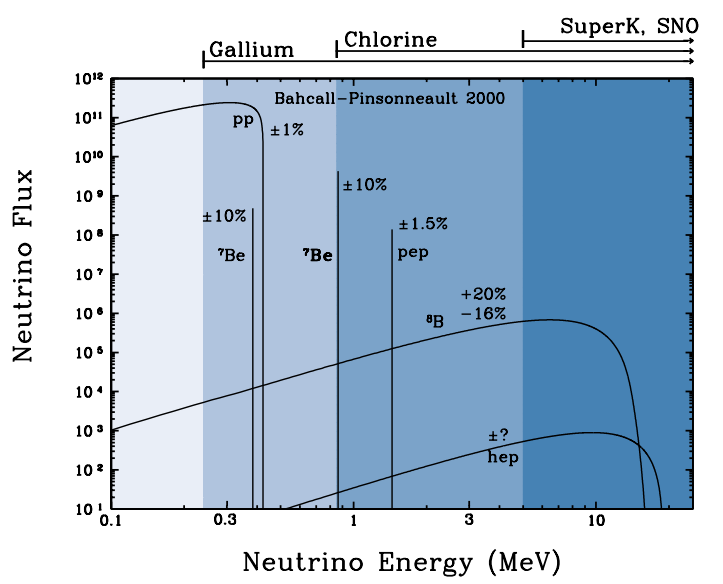
\includegraphics[height=90mm]{Chapter1/Figs/Raster/neutrino_emmision_graph.png}
 \captionof{figure}{The solar neutrino spectra predicted by the SSM. The neutrino fluxes at one astronomical unit from continuum sources are given in units of cm$^{-2}$ s$^{-1}$ MeV$^{-1}$ , and the line fluxes are given in cm$^{-2}$ s$^{-1}$ from \cite{Bellerive:2003rj}} %~can be used as a kind of place holder in latex
 \label{neutrino_emmision_graph}
\end{figure}
\begin{equation}
    \nu + e \rightarrow  \nu + e
    \label{neutrino_scattering}
\end{equation}
\begin{equation}
    \nu_e + d \rightarrow p + p + e 
    \label{charged-current_reaction}
\end{equation}
\begin{equation}
    \nu + d \rightarrow  n + p + \nu
    \label{neutral-current_reaction}
\end{equation}
\\By combining the results from the SuperK which uses exclusively neutrino scattering, equation \ref{neutrino_scattering}, and SNO results for CC results using equation \ref{charged-current_reaction} it is possible to solve the solar neutrino problem. SuperK found 45.1 $\pm$ 0.5 (stat)$^{+1.6}_{-1.4}$ (syst)\,\% according to the BP2000 standard solar model \cite{superK2001}. Whereas the CC results, equation \ref{charged-current_reaction}, from SNO found 34.7 $\pm$ 2.9\,\% of the $\nu_e$ expected as seen in figure \ref{sno_superK_comparision_plot} \cite{sno2001}. There is a $\sim$ 10\,\% discrepancy between these two results. But this does not mean 10\,\% of the neutrinos were $\nu_\mu$ and $\nu_\tau$, as the SuperK detector is 6.5 times more sensitive to $\nu_e$ so 10\,\% $\times$ 6.5 = 65\,\% of the neutrinos are $\nu_\mu$ and $\nu_\tau$. And so all neutrinos are now accounted for and thus the solar neutrino problem was deemed solved \cite{griffiths2008book} \cite{griffiths2008neutrinoOscillations}.

%\cite{Ashenfelter:2015tpm} %prospect citation

\begin{figure}[htbp]
 \centering
 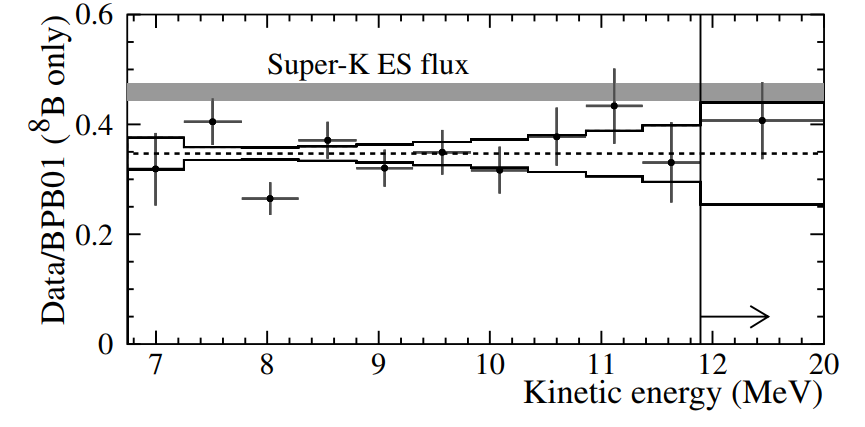
\includegraphics[height=75mm]{Chapter1/Figs/Raster/superKSnoComparison.png} %height of this plot had to be adjusted because of its unusal diemensions
 \captionof{figure}{The ratio of the data to the expected kinetic energy distribution with correlated systematic errors for the $^8$B charged current interactions. Notice the $\sim$ 10 \,\% discrepancy in data between the super K elastic scattering flux (in shaded grey) and the SNO charged current flux (the dashed line). From \cite{sno2001}} %~can be used as a kind of place holder in latex
 \label{sno_superK_comparision_plot}
\end{figure}


%\begin{figure}[htbp]
% \centering
% 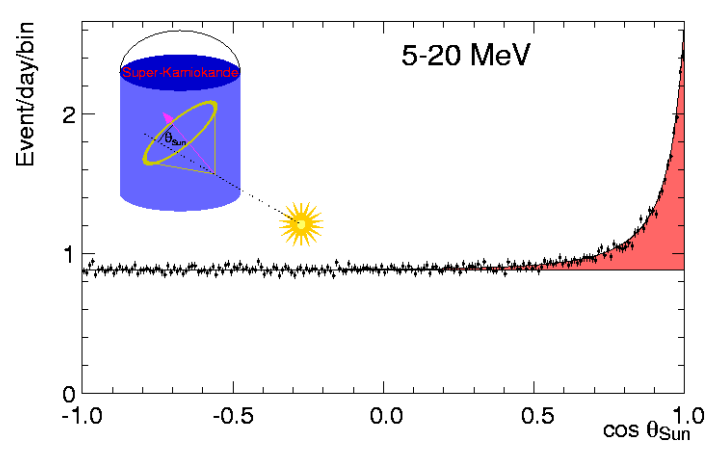
\includegraphics[height=90mm]{sk_angular_neutrinos.png}
% \captionof{figure}{from \cite{Bellerive:2003rj}} %~can be used as a kind of place holder in latex
% \label{sk_angular_neutrinos}
%\end{figure}

\subsection{Neutrino oscillations} \label{section_neutrino_oscillations}
% Neutrino oscillations were proposed in 1968 after the Davis experiment \cite{davis1968homestake}. A man called Pontecorvo discussed the possibility of oscillations in 1957 and revived the idea in 1968 as a solution to the solar neutrino problem \cite{griffiths2008book}\cite{griffiths2008neutrinoOscillations}. With the original 1958 paper being \cite{pontecorvo1958_OscillationProposal}, suggesting the transformation of Kiaons. And the suggestion for the solution to the solar neutrino problem being here \cite{pontecorvo_gibov_1969_solar_oscillation}. Note these are a little hard to get hold of but some old russian servers still have them, Googling not too hard. 
% \\Most of this section will follow \cite{griffiths2008book} \cite{griffiths2008neutrinoOscillations}. There is a more in depth explanation using \cite{sassaroli1999neutrino} in which \cite{griffiths2008book} \cite{griffiths2008neutrinoOscillations} follows the standard treatment for neutrino oscillations. \cite{sassaroli1999neutrino} also goes through a relativistic treatment but that's probably too much for this overview and not really necessary for explaining the phenomena of oscillations, it should still be mentioned though. Wavelength of neutrino and kaon oscillations mentioned before are outlined by \cite{burkhardt2003wavelength}, it goes through the kinematics and shows that the oscillations do account for the mass difference, again quite in depth maybe overkill... should talk to one of my supervisors about this... 
% \\Also there is the MSW (named after the people who found it) effect however the exact papers appear to be a bit difficult to find but I was able to get something very detailed from Mikheev 1987 which goes into interactions with matter \cite{Mikheev_1987}.
Oscillations had been proposed in 1958 with regards to $K^0$/$\Bar{K^0}$ as an analogy to the possibility of $\nu$/$\Bar{\nu}$ oscillations \cite{griffiths2008book} \cite{griffiths2008neutrinoOscillations} \cite{pontecorvo1958_OscillationProposal}. When the Davis and Harmer experiment in 1968 produced a lack of neutrinos in comparison to the standard solar model the idea of neutrino oscillations was revived to explain this discrepancy \cite{pontecorvo_gibov_1969_solar_oscillation}. At the time the reactor monitoring experiments excluded an oscillation length smaller than a few metres but to measure the true oscillation length would require measuring the neutrino production from the sun. This was due to the lengths involved \cite{pontecorvo_gibov_1969_solar_oscillation} and as seen in table \ref{solar_nuetrino_table} the production mechanisms for solar neutrinos are all $\nu_e$s so if any oscillations occur a discrepancy would be visible. 
\\
\begin{table*}
\centering
\begin{tabular}{lllll}  
\toprule
\multicolumn{1}{c}{Reaction} & \multicolumn{1}{c}{Label} & \multicolumn{1}{c}{Flux [cm$^{-2}$s$^{-1}$]}
\\
\cmidrule(r){1-1}
\cmidrule(r){2-2}
\cmidrule(r){3-3}
p+p $\rightarrow$ $^2$H+e$^+$+$\nu_e$           & pp                & 5.95 $\times$ 10$^{10}$\\
p+e$^-$+p$\rightarrow$ $^2$H+ $\nu_e$           & pep               & 1.40 $\times$ 10$^{8}$\\
$^3$He+p $\rightarrow$ $^4$He+e$^+$+ $\nu_e$     & hep               & 9.3  $\times$ 10$^{3}$\\
$^7$Be+e$^-$ $\rightarrow$ $^7$Li+ $\nu_e$       & $^7$Be            & 4.77 $\times$ 10$^{9}$\\
$^8$B $\rightarrow$ $^8$Be$^*$+e$^+$+ $\nu_e$   & $^8$B             & 5.05 $\times$ 10$^{6}$\\
\bottomrule   
\end{tabular}
\caption{Neutrino production from fusion reactions in the Sun from \cite{Bellerive:2003rj} }
\label{solar_nuetrino_table}
\end{table*}
\\\\In order to predict the number of neutrinos that are supposed to oscillate between one form and another there are two approaches that can be taken, the first approach is to treat the two system as a linear combination of eigenstates $\nu_e$ $\nu_\mu$ \cite{griffiths2008book}\cite{griffiths2008neutrinoOscillations} \cite{sassaroli1999neutrino}. Then there is the full quantum mechanical treatment of neutrino oscillations which uses ``Diagonalization of the two coupled direc equations'' and ``Field quantization, anticommutation relations and flavor wave functions'' \cite{sassaroli1999neutrino}. The following approach will use a linear combination of eigenstates which is considered the ``standard treatment'' \cite{sassaroli1999neutrino} \cite{griffiths2008book} \cite{griffiths2008neutrinoOscillations}.
\\\\Let's begin with two eigenstates with $\nu_1$ and $\nu_2$: 
\begin{equation}
    \begin{bmatrix}
        \ket{\nu_1} \\
        \ket{\nu_2}
    \end{bmatrix}
    =
    \begin{bmatrix}
        \cos\theta & -\sin\theta \\
        \sin\theta & \cos\theta 
    \end{bmatrix}
        \begin{bmatrix}
        \ket{\nu_e} \\
        \ket{\nu_\mu}
    \end{bmatrix}
    \label{linear_combination_eq_1}
\end{equation}
We then introduce $C_e$ and $C_\mu$ which are the amplitudes for detecting an electron neutrino and a muon neutrino, respectively. And introduce $C_1$ and $C_2$ which are the amplitudes for finding the neutrino in the energy states $E_1$ and $E_2$ , respectively. The coefficients $C_1$ and $C_2$ evolve over time as:
\begin{equation}
    C_1(t) = C_1(0)e^{-iE_1t}, \quad  C_2(t) = C_2(0)e^{-iE_2t}
    \label{linear_combination_eq_1.5}
\end{equation}
Which we know from the schrodinger equation \cite{sassaroli1999neutrino} \cite{griffiths2008book}\cite{griffiths2008neutrinoOscillations}. We then introduce the the rotation matrix between the flavor and mass eigenstates (equation \ref{linear_combination_eq_1}) then the following relation between the energy and flavor amplitude holds:
\begin{equation}
    \begin{bmatrix}
        C_1(t) \\
        C_2(t)
    \end{bmatrix}
    =
    \begin{bmatrix}
        \cos\theta & -\sin\theta \\
        \sin\theta & \cos\theta 
    \end{bmatrix}
        \begin{bmatrix}
        C_e(t) \\
        C_\mu(t)
    \end{bmatrix}
    \label{linear_combination_eq_2}
\end{equation}
By then multiplying by the inverse of the sine cosine matrix and substituting in using equation \ref{linear_combination_eq_1.5} the following relation follows:
\begin{equation}
    \begin{bmatrix}
        C_e(t) \\
        C_\mu(t)
    \end{bmatrix}
    =
    \begin{bmatrix}
        \cos\theta & -\sin\theta \\
        \sin\theta & \cos\theta 
    \end{bmatrix}
        \begin{bmatrix}
        C_1(0)e^{-iE_1t} \\
        C_2(0)e^{-iE_2t}
    \end{bmatrix}
    \label{linear_combination_eq_3}
\end{equation}
We now impose a boundary condition in order to get a given flavour production. Let us say that at time 0 a muon netrino is produced this corresponds to:
\begin{equation}
    C_\mu(0) = 1, \quad C_e(0) = 0
    \label{linear_combination_eq_4}
\end{equation}
By putting these values into equation \ref{linear_combination_eq_2} the following is obtained:
\begin{equation}
    C_1(0) = -\sin\theta, \quad C_2(0) = \cos\theta
    \label{linear_combination_eq_5}
\end{equation}
In order to get the time evolution of the flavour amplitudes equation \ref{linear_combination_eq_5} is substituted into equation \ref{linear_combination_eq_3} in order to receive the following relations for electron and muon neutrinos: 
\begin{equation}
    C_e(t)=\sin\theta\cos\theta(e^{-iE_2t}-e^{-iE_1t})
    \label{linear_combination_eq_6}
\end{equation}
\begin{equation}
    C_\mu(t)=\sin^{2}e^{-iE_1t} + \cos^{2}e^{-iE_2t}
    \label{linear_combination_eq_7}
\end{equation}
%side note what is l I think griffiths talks about it...
Space and momentum are then introduced: 
\begin{equation}
   E_1^2=m_1^2 + p^2, \quad E_2^2=m_2^2  , \quad L \approx t
    \label{linear_combination_eq_8}
\end{equation}
Note that L is actually $\approx ct$ but in the following $c$ is assumed to be 1 and therefore not written. Thus the probability for the neutrino flavour oscillations between muon and electron neutrinos is as follows: 
\begin{equation}
   {\mid{C_e}\mid}^2 = \sin^2(2\theta)\sin^2[(E_2-E_1)t/2] \approx \sin^2(2\theta)\sin^2\left[\frac{(m_1^2-m_2^2)L}{4E}\right]
    \label{linear_combination_eq_9}
\end{equation}
\begin{equation}
    {\mid{C_\mu}\mid}^2 = 1 - \sin^2(2\theta)\sin^2[(E_2-E_1)t/2] \approx 1 - \sin^2(2\theta)\sin^2\left[\frac{(m_1^2-m_2^2)L}{4E}\right]
    \label{linear_combination_eq_10}
\end{equation}
Note that for equations \ref{linear_combination_eq_9}, \ref{linear_combination_eq_10} $E = p$, these equations also have to be averaged over the energy distribution of particles involved. Also the assumption that the muon neutrino is created with a definite momentum p is only an approximation \cite{sassaroli1999neutrino}. This explanation follows \cite{sassaroli1999neutrino} which also gives the full quantum mechanical treatment as well. If we take equation \ref{linear_combination_eq_9} we can see that at a distance $L = (4E\pi) / (m_1^2 - m_2^2)$ there will be a maximum conversion to electron neutrinos and at $2L$ there will be a maximum conversion to muon neutrinos. 

\subsection{Mixing Angles}
% Firstly it would be a good idea to pull from \cite{griffiths2008book}\cite{griffiths2008neutrinoOscillations} which does mention that according to equations \ref{linear_combination_eq_9} and \ref{linear_combination_eq_9} the masses must be unequal and cannot be zero. i.e. $m_i \neq m_j$ and $\Delta m_\theta \neq 0$. \\
% The review of particle physics 2014 is probably quite useful here\cite{Olive_2014}, this may also start to bleed into the other sections, results from T2K, dayabay, double CHOOZ and KamLand may need to be added here. As this is quite a difficult section, lot of potential pit falls and I need to make sure the info I give is up to date because the information is changing frequently. 
% \\I need to show the neutrino mixing matrix and how the dirac and Majorana components work with the mixing angles as shown below (the PMNS matrix) 
% \begin{equation}
% U
%     =
%     \begin{bmatrix}
%         c_{12}c_{13} & s_{12}c_{13} & s_{13}e^{-i\delta}\\
%         -s_{12}c_{23} - c_{12}s_{23}s_{13}e^{i\delta} & c_{12}c_{23} - s_{12}s_{23}s_{13}e^{i\delta} & s_{23}c_{13} \\
%         s_{12}s_{23} - c_{12}c_{23}s_{13}e^{i\delta} & -c_{12}s_{23} - s_{12}c_{23}s_{13}e^{i\delta} & c_{23}c_{13} 
%     \end{bmatrix}
%     \\ \times \text{diag}(1, e^{\frac{i\alpha21}{2}} , e^{\frac{i\alpha31}{2}})
%     \label{neutrino_mixing_matrix}
% \end{equation}
% The dirac CP violation phases are represented by the $\delta$ components the Majorana CP violation is represented by the $\alpha$ components this was taken from \cite{Olive_2014}, which extrapolated it from \cite{Bilenky_1980}, \cite{Schechter_and_Valle_1980} both of which are heavily cited articles themselves.It may be a good idea to mention the CKM quark mixing matrix too. and also cite it. 
% \\I also need to cite double chooz whilst \cite{Olive_2014} has a good handle on $\theta_{12}$ (solar) and $\theta_{23}$ (atmosphere) the value of $\theta_{13}$ (reactor) was before the latest results of the double chooz experiments. So I need to hunt down there most recent paper of which I found was \cite{abe2014improved}, but that was in 2014... It is also worth pointing out as \cite{Olive_2014} does that the oscillations for neutrinos will be very different to the oscillations that quarks undergo these mixing angles are very different. Also worth pointing out that so far no evidence for Majorana neutrinos has be found. Mention neutrino-less double $\beta$ decay as a possibility for Majorana neutrinos or at least an exclusion of dirac neutrinos \cite{Schechter_and_Valle_1982}. latest. 
According to equations \ref{linear_combination_eq_9}, \ref{linear_combination_eq_10} for oscillations to occur there must be mass differences between the two neutrino types. If neutrinos were mass-less then the oscillations could not occur as the values for the probabilities would be zero according to equations \ref{linear_combination_eq_9}, \ref{linear_combination_eq_10}. Therefore the existence of neutrino oscillations shows that the assumption of mass-less neutrinos is incorrect \cite{griffiths2008book}\cite{griffiths2008neutrinoOscillations} \cite{sassaroli1999neutrino}. There are three different types of neutrino: $\nu_e$, $\nu_\mu$ and $\nu_\tau$. These neutrinos interact as flavor eigensates, they propagate as eigenstates of the free-particle Hamiltonian - the mass eigenstates $\nu_1$, $\nu_2$ and $\nu_3$. The flavour mass eigenstates evolve complexly due to the three different masses contributing to the pattern  \cite{griffiths2008book} \cite{griffiths2008neutrinoOscillations}. 
\\\\These flavour changes can be represented by three different angles $\theta_{12}$ ($\theta_{sol}$), $\theta_{23}$ ($\theta_{atm}$), $\theta_{13}$ ($\theta_{reactor}$) \cite{Olive_2014} \cite{griffiths2008book} \cite{griffiths2008neutrinoOscillations}. These angles can be represented by the following  matrix in equation \ref{PMNS_matrix} which is referred to as the Pontecorvo–Maki–Nakagawa–Sakata (PMNS) matrix
\begin{equation}
U
    =
    \begin{bmatrix}
        c_{12}c_{13} & s_{12}c_{13} & s_{13}e^{-i\delta}\\
        -s_{12}c_{23} - c_{12}s_{23}s_{13}e^{i\delta} & c_{12}c_{23} - s_{12}s_{23}s_{13}e^{i\delta} & s_{23}c_{13} \\
        s_{12}s_{23} - c_{12}c_{23}s_{13}e^{i\delta} & -c_{12}s_{23} - s_{12}c_{23}s_{13}e^{i\delta} & c_{23}c_{13} 
    \end{bmatrix}
    \\ \times \text{diag}(1, e^{\frac{i\alpha21}{2}} , e^{\frac{i\alpha31}{2}})
    \label{PMNS_matrix}
\end{equation}
Where $s_{ij}$ and $c_{ij}$ represent $\sin(\theta_{ij})$ and $\cos(\theta_{ij})$ respectively. The equation is also parametrised by the CP violation phases $\delta$ and $\alpha$ which represent the Dirac and Majorana phases respectively \cite{Olive_2014}. However at this time experiments to prove the Majorana over Dirac neutrinos have not proven fruitful as neutrino-less double $\beta$ decay has not been observed due to the challenging theoretical and experimental requirements (though experiments are improving their precision) \cite{Cardani_2019}.  So the above PNMS matrix is often written without the Majorana component ($\text{diag}(1, e^{\frac{i\alpha21}{2}} , e^{\frac{i\alpha31}{2}})$). 
\\\\The narrowing of the mixing angles has been ongoing in neutrino physics. As a result there are many experiments that have contributed to the improvements in angles which can be seen in figure \ref{neutrino_angles_experiments_variations} 
 which shows the regions favoured or excluded by the oscillation experiments. The measurement of solar neutrinos and the resulting solar neutrino problem has already been covered. And due to the abundance of solar neutrinos the angle $\theta_{12}$ has been measured frequently as seen in figure \ref{neutrino_angles_experiments_variations}. There are also also an abundance of terrestrial $\nu_\mu$s which are produced in the atmosphere from cosmic proton interactions which in turn produce pions which decay into muons and $\nu_\mu$ \cite{griffiths2008book}\cite{griffiths2008neutrinoOscillations}.
\begin{equation}
    \pi^+ \rightarrow \mu^+ + \nu_\mu,\quad \mu^+ \rightarrow e^+ + \nu_e + \Bar{\nu}_\mu 
    \label{pi_plus_neutrino_production}
\end{equation}
\begin{equation}
    \pi^- \rightarrow \mu^- + \nu_\mu, \quad \mu^- \rightarrow e^- + \nu_e + \Bar{\nu}_\mu 
    \label{pi_minus_neutrino_production}
\end{equation}
\begin{figure}[htbp]
 \centering
 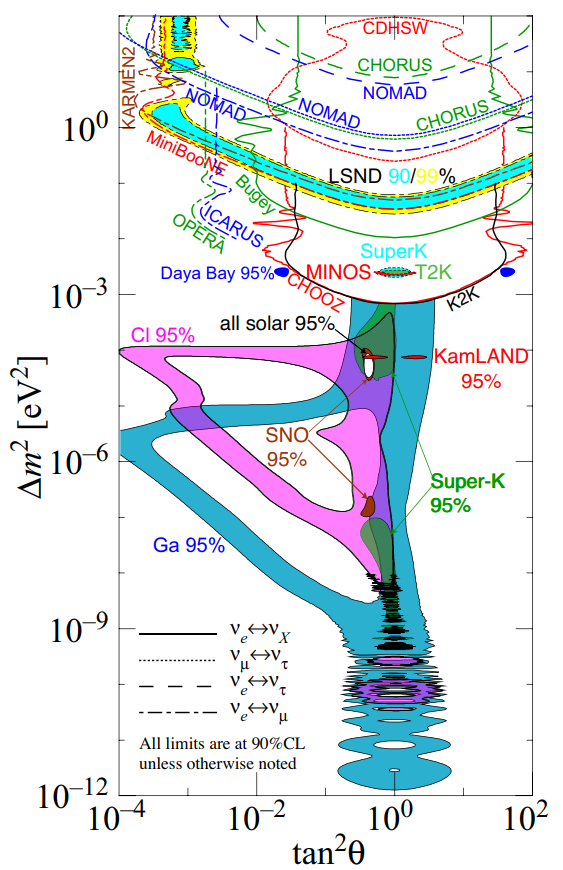
\includegraphics[height=150mm]{Chapter1/Figs/Raster/neutrino_angles_experiments_variations.png} %height of this plot had to be adjusted because of its unusal diemensions
 \captionof{figure}{The regions of squared-mass splitting and mixing angle favoured or excluded by various experiments based on two-flavor neutrino oscillation analyses. References to the data can be found at \url{http://hitoshi.berkeley.edu/neutrino} from \cite{Olive_2014}} %~can be used as a kind of place holder in latex
 \label{neutrino_angles_experiments_variations}
\end{figure}
Therefore from  has been an increase in the number of experiments measuring $\theta_{13}$ however due to the production of $\nu_e$s from the sun this presents a unique challenge \cite{Olive_2014}. The solution is to use reactor produced $\Bar{\nu_e}$s at a baseline of $\sim$ 1\,km such that oscillations driven by $\Delta m_\odot^2$ are negligible. The first experiment to do this was the chooz experiment, however it was unable to find any evidence of $\Bar{\nu_e}$ disappearance \cite{Olive_2014}. However the experiment was revised into the double Chooz experiment which has been able to measure $\Bar{\nu_e}$ disappearance and thus measure $\theta_{13}$ with $\sin^22\theta_{13} = 0.090^{+0.032}_{-0.029}$ when fitting to spectrum \cite{abe2014improved}. RENO and Daya Bay have also measured $\Bar{\nu_e}$ disappearance and $\theta_{13}$ as well \cite{Olive_2014}.  

\section{Sterile Neutrinos}
    Leave this for another time... its its own can of worms... 5MeV bump and monitoring stuff

\section{Anti-neutrino Reactor Monitoring}
% Obviously the two papers to mention here are vogal and beacom 1999 \cite{Vogel_1999} and muller et al 2011 \cite{Mueller_2011}. They cover the ground pretty well. \cite{Mueller_2011} has the $10^{20}$ $\Bar{\nu_e}$/s per GW$^{Th}$ and \cite{Vogel_1999} has the cross section values. \cite{Vogel_1999} is mostly dealing with stuff to first order, it may be worth addressing how this changes with increasing order. But probably not considering the low number of events anti-neutrino detection yields. Worth also going over the cowan and riens \cite{Cowan1956Confirmation} \cite{cowan1957test} again just briefly. The songs s1 project is also a necessity in 2007 it marked the beginning of serious reactor monitoring \cite{Bowden_2007}. And of course the original soviet paper which suggested this is as a possibility \cite{Borovoi_1978}. Also need to mention the IAEA and there workshop which suggested the limitations for this \cite{IAEA_2008}. 
% \\\\Probably best to go onto semi chronologically with the Cowan and Reins approach stating that reactor monitoring was one of the original approaches as fuel decays through beta decay (equation \ref{modern_beta_decay}) and the detection occurs through equation \ref{inverse_beta_decay}. It may be worth also mentioning section \ref{Direct_Measurements_section}. Then mentioning the soviet paper \cite{Borovoi_1978} then the move on to the first prototype with SONGS1 and then \cite{Bowden_2007} which then informed the IAEA report \cite{IAEA_2008}. Then talk about vogel \cite{Vogel_1999} and muller \cite{Mueller_2011}.
As mentioned earlier in section \ref{Direct_Measurements_section} an attempt to measure anti-neutrinos from reactors was the first method to prove anti-neutrinos existed. By measuring the response of anti-neutrinos in cadmium doped liquid scintillation detector \cite{Cowan1956Confirmation}. Which used inverse $\beta$ decay (equation \ref{inverse_beta_decay}). $\sim$ 20 years after the experiment using anti-neutrinos from reactors was suggested for reactor monitoring in 1978 \cite{Borovoi_1978}. However due to the geopolitics of the time, the interest in non-proliferation was not as high as in modern times. It took until 2007 for the SONGS1 prototype to be deployed as proof of concept for reactor monitoring \cite{Bowden_2007}. 
\\\\After the deployment of the SONGS1 prototype the IAEA issued a list of positive traits the organisation would like in an anti-neutrino reactor monitoring detector: inert construction, non-liquid, easy operation, cheap, portable, robust, above ground operation, easy deployment \cite{IAEA_2008}. Whilst these are not requirements all of these traits can be met in a single detector. For example VIDARR meets all of these traits. 
\\\\Reactors produce $10^{20}$ $\Bar{\nu_e}$/s per GW$^{Th}$ as the fission products in the fuel elements $\beta$ decay \cite{Mueller_2011}. Though these statistics are very high the interaction cross section to first order is $\sim$ $10^{-42}$cm$^2$ as can be seen in figure \ref{vogelAndBeacomCrossSection} \cite{Vogel_1999}. In addition to this different fission fractions will decay at different rates as can be seen in figure \ref{mullerAndVogelCombined}. The combination of these two effects can be seen in figure \ref{mullerEtAlDetectedSpectrum} \cite{Mueller_2011}. This means that a detected spectrum of $\Bar{\nu_e}$s are only visible between $\sim$ 1.5\,MeV and $\sim$ 8.5\,MeV as can be seen in figure \ref{mullerEtAlDetectedSpectrum}. 
\begin{figure}[htbp]
 \centering
 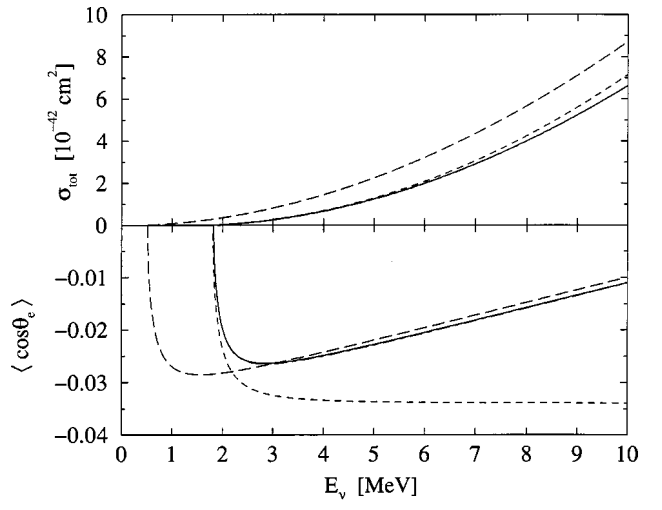
\includegraphics[width=120mm]{Chapter1/Figs/Raster/vogelAndBeacomCrossSection.png} %height of this plot had to be adjusted because of its unusal diemensions
 \captionof{figure}{Upper panel: total cross section for Inverse $\beta$ decay; bottom panel: $\bra{}\cos(\theta)\ket{}$ for the same reaction; both as a function of the anti-neutrino energy. The solid line is the O(1/M) result and the short-dashed line is the O(1) result. The long-dashed line is the result of Eq. 3.18 from \cite{smith_1972}. \cite{Vogel_1999}} %~can be used as a kind of place holder in latex
 \label{vogelAndBeacomCrossSection}
\end{figure}
\begin{figure}[htbp]
 \centering
 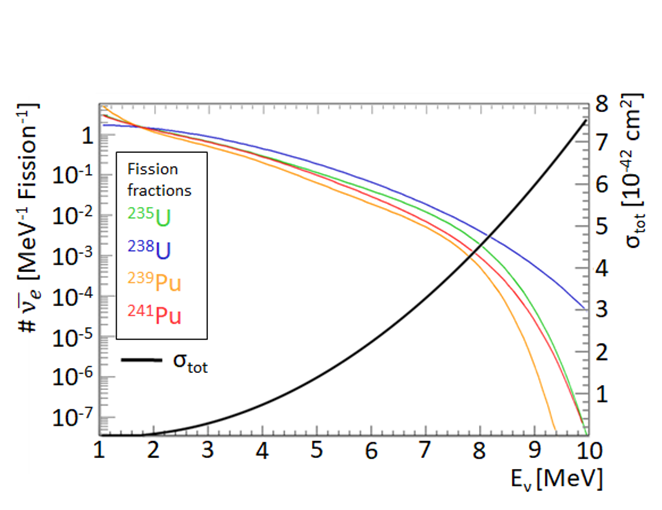
\includegraphics[height=75mm]{Chapter1/Figs/Raster/mullerAndVogelCombined.png} %height of this plot had to be adjusted because of its unusal diemensions
 \captionof{figure}{A combination of the fission fractions from \cite{Mueller_2011} and the first order approximation of the cross section from \cite{Vogel_1999} and how they evolve over the energy range where the two distributions cross over.} %~can be used as a kind of place holder in latex
 \label{mullerAndVogelCombined}
\end{figure}
\begin{figure}[htbp]
 \centering
 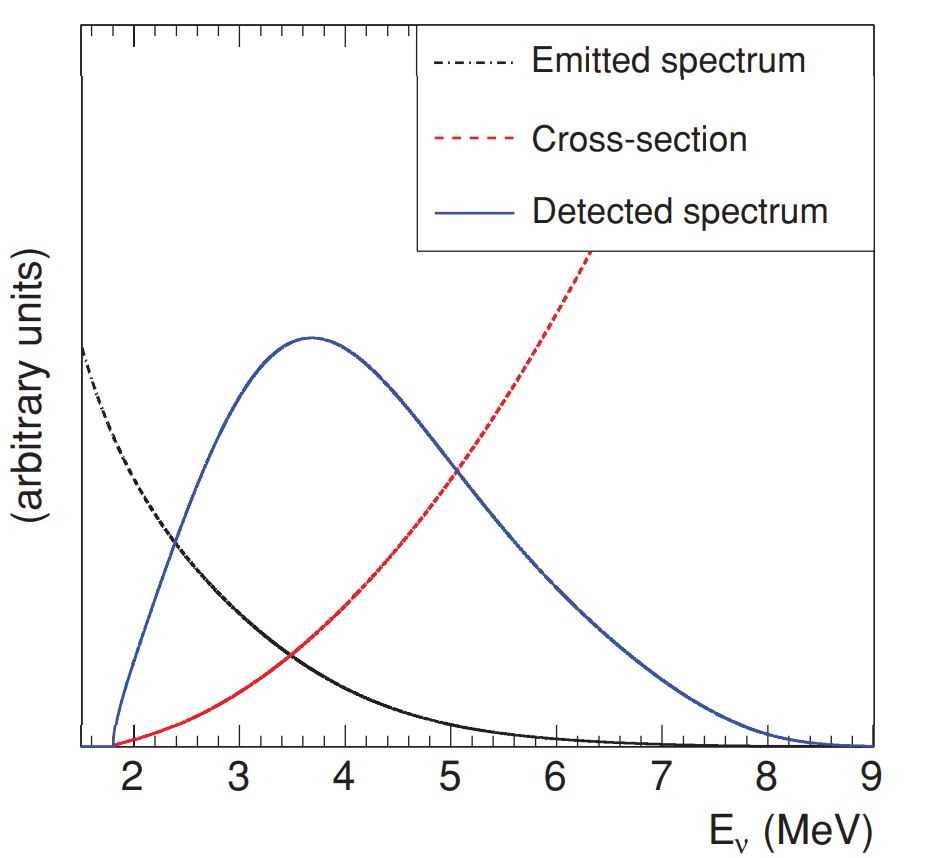
\includegraphics[height=75mm]{Chapter1/Figs/Raster/mullerEtAlDetectedSpectrum.png} %height of this plot had to be adjusted because of its unusal diemensions
 \captionof{figure}{Colour online) Detected anti-neutrino spectrum for $^{235}$U fission (blue solid curve). Units are arbitrary and oscillation effects are suppressed. The detected rate rises from the threshold value at about 1.8\,MeV, reaches a maximum around 4\,MeV, and vanishes after 8\,MeV. This shape is the result of folding the emitted spectrum (black dashed-dotted curve), parametrization taken from \cite{Mueller_2011} Sec. V A and inverse $\beta$ cross section (red dashed curve). \cite{Mueller_2011}} %~can be used as a kind of place holder in latex
 \label{mullerEtAlDetectedSpectrum}
\end{figure}
\\\\It may be possible to discern the different fission fraction isotopes from their detected spectra. Providing the energy resolution and statistics of the detector and location are sufficient. This would be very useful for non-proliferation purposes as measuring the Pu$^{239}$ burn up would lead to a more accurate measure of weapons grade material than on off cycles would provide. As online refuelling methods seen in reactors such as the Advanced Gas cooled Reactors (AGRs) would not work around the measurement of Pu$^{239}$ burn-up. 



\ifpdf
    \graphicspath{{Chapter1/Figs/Raster/}{Chapter1/Figs/PDF/}{Chapter1/Figs/}}
\else
    \graphicspath{{Chapter1/Figs/Vector/}{Chapter1/Figs/}}
\fi




